% !TEX root = ../Tesi_Triennale_PMNS.tex
\chapter{Analisi}
\label{chapter:analisi}
\section{Primo approccio all'algoritmo}
\label{section:analisiSimSingole}
\begin{center}
	$\smallsim 2/3$ pagine
\end{center}
	
\begin{center}
	\begin{figure}[H]
		\centering
		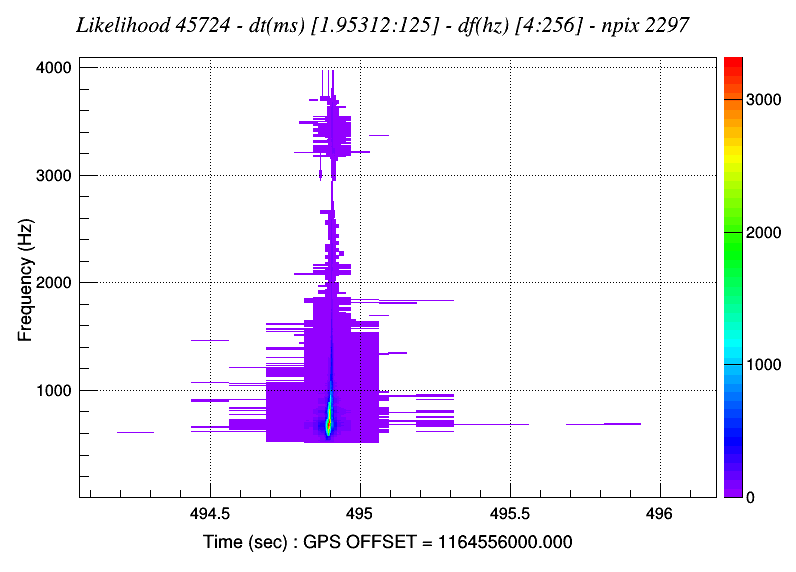
\includegraphics[scale=0.38, angle=0]{figures/Capitolo_4/APR4_q09/layer4_10__distance5_1250_2500_5000/ced_1164556010_790_O4I_GN_LHV_SIM_PMNS_APR4_q09_NEW_4_job1/L1H1V1_1164556494.250_1164556494.250_1164556494.250/l_tfmap_scalogram.png}
		\setlength{\belowcaptionskip}{-20pt}
		\caption{}
		\label{fig:APR4q09/likelihood}
	\end{figure}
\end{center}	
\subsection{APR4q09}



\subsection{SHT2.0spinf1}

\subsection{SHT2.2spinf1}


\lipsum[7]\cite{hartle2003gravity}.

\section{Ricerca frequenza post-merger}
\begin{center}
	$\smallsim 5/6$ pagine
\end{center}

\begin{center}
	\begin{figure}[H]
		\centering
		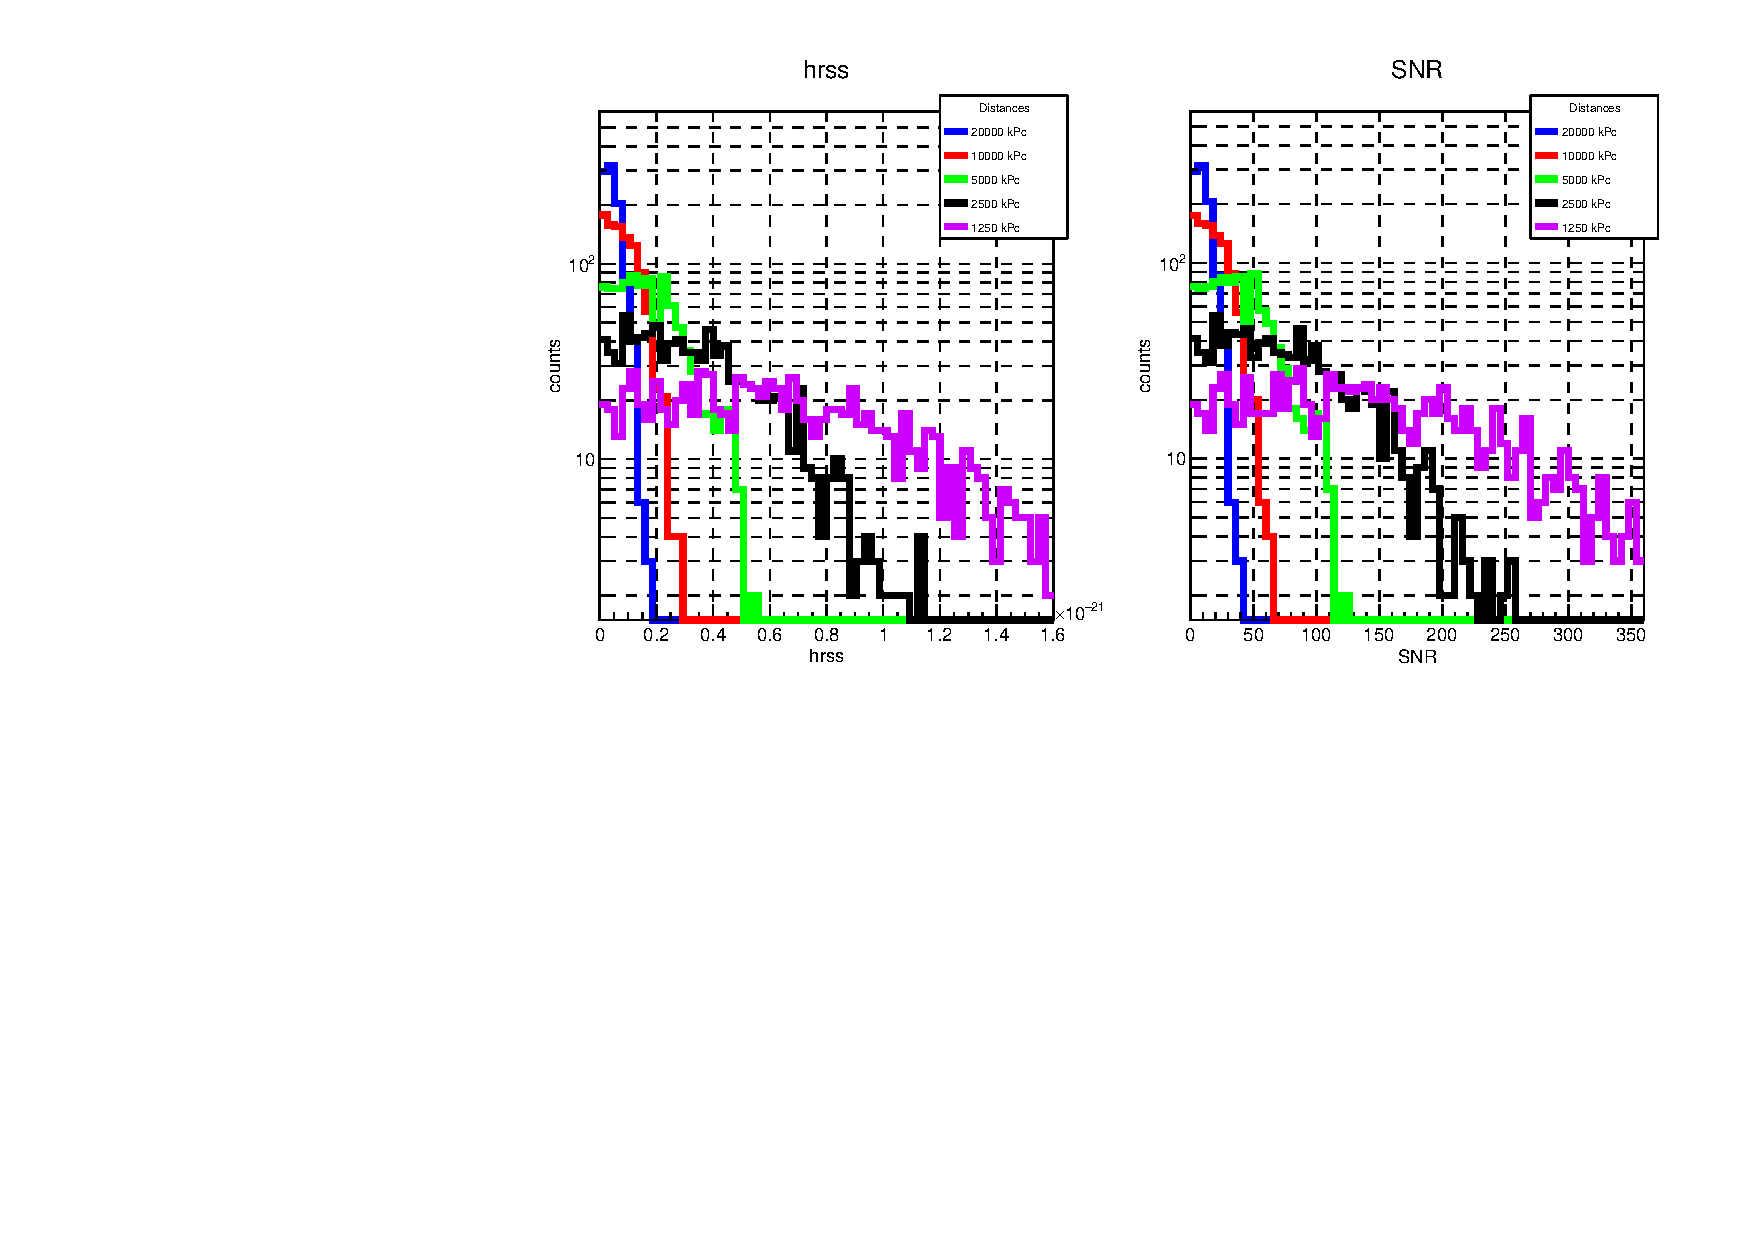
\includegraphics[scale=0.68, angle=0]{figures/Capitolo_4/hrss_snr_Distribution.pdf}
		\setlength{\belowcaptionskip}{-20pt}
		\caption{}
		\label{fig:hrss_snr_distribution}
	\end{figure}
\end{center}	


\lipsum[8]

\lipsum[9]